% In the batch queue,  queue time becomes dominant but, at the same time, we
% have more freedom to decide the parameters of the slot.

\subsection{Experiments}

In this section we present experiments that aim to determine the performances of the NGE and to show how it provides a minimal overhead while introducing new functionalities.

Experiments consist in running AthenaMP instances by using NGE pilots where each AthenaMP simulates a pre-determined number of events taken from ATLAS workload.	
We present four groups of experiments in which we test the NGE for weak scalability, weak scalability with resubmission, strong scalability and heterogeous workloads.

We collect data about the execution time of the pilots and the AthenaMP that are executed within them by considering all stages that these entities pass through during the execution.
Experiments have been performed out of production by using NGE's pilots on TITAN's batch queue. 
Because of TITAN's batch queue, the turnaround time of each run of our experiments is dominated by the time spent on TITAN's queue. Since we are interested only in the performances of the NGE, we removed queue time from our statistics.

All the experiments have been performed by setting AthenaMP in such a way that it uses all the 16 cores present on TITAN's nodes. 


\subsubsection{Weak scalability}

The experiment consists in running as many AthenaMP instances (also referred as tasks from now-on) as the number of nodes controlled by the pilot. Each AthenaMP have been assigned with 100 events whose simulation requires  ~$80$ minutes. 
 
Tasks do not experience queue within the pilot since there is one node for each AthenaMP instance. Therefore, delays are consequence of only three factors: i) the bootstrapping of the pilot on the nodes; ii) the manager, as defined in Section \ref{}, that has to dispatch tasks to the pilot; iii) the time that the agent requires to spawn all the tasks on the nodes.

We tested different pilot sizes, i.e. : 250, 500, 1000 and 2000. For all of them the walltime was 2 hours.

Figure \ref{fig:weakScal1a} depicts the average pilot duration and the average execution time of AthenaMP as function of the pilot size.  

\begin{figure}[!htb]
        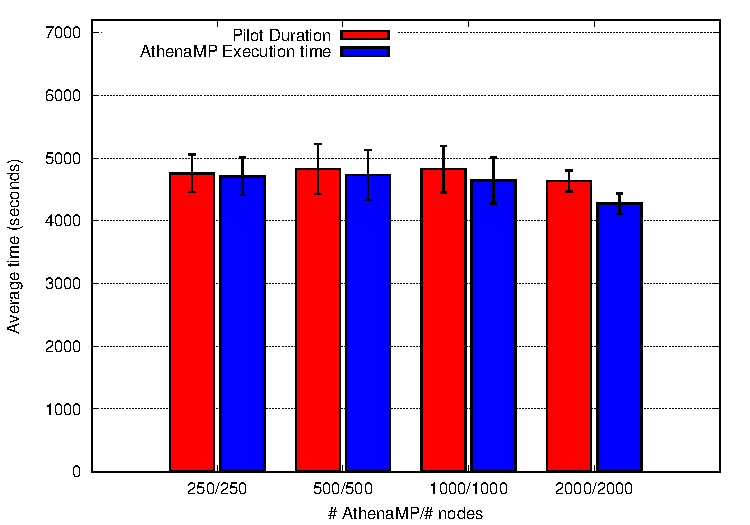
\includegraphics[width=0.5\textwidth]{./figures/NGE/weakET1.pdf}
    \caption{Average pilot execution time against average AthenaMP execution times for pilot sizes: 250, 500, 1000 and 2000.}
\label{fig:weakScal1a}
\end{figure}

On the one side, we can observe that the average pilot duration is insensitive to the pilot size. This indicates that, on average, the overhead introduced by the pilot does not grow significatively with the size of the pilot.
On the other side, we can notice that the average execution time of AthenaMP is smaller than the average pilot duration. This indicates that the overhead of the pilot is not null and can be quantified in ~5 minutes.  

\aanote{I think we should say something about the execution time of AthenaMP that is smaller than the others.}

In Figure \ref{fig:weakScal1b}, we provide the time required by the pilot to start running AthenaMP instances.  
We can notice that the larger is the number of units and the larger is the time required by the pilot to start running them. However, we can observe that the time does not grow linearly with the pilot size. 

\begin{figure}[!htb]
        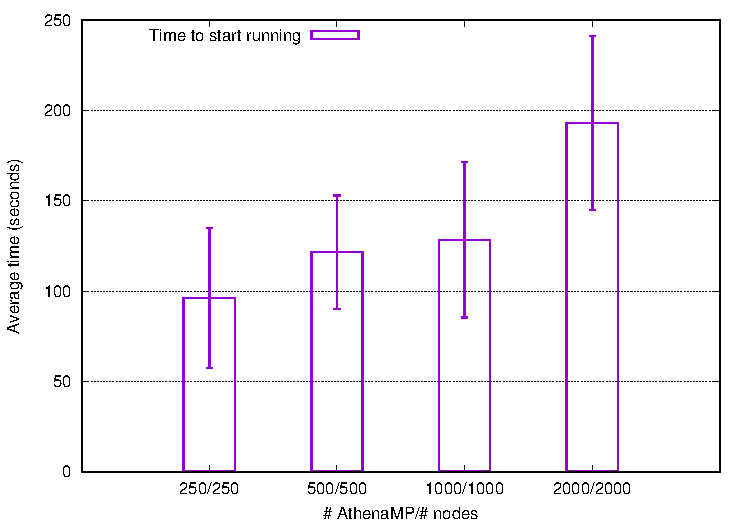
\includegraphics[width=0.5\textwidth]{./figures/NGE/weakStart1.pdf}
    \caption{Average time to start running AthenaMP for pilot sizes: 250, 500, 1000 and 2000.}
\label{fig:weakScal1b}
\end{figure}


\subsubsection{Weak scalability with resubmission }
This experiment is similar to the one presented above but in this case we want to test also the impact of submitting new AthenaMP instances in place of those that end. The reason behind this experiment is to stress pilot's components by pushing new tasks while others are ending their execution.

In order to perform the experiments in less than two hours per run, we decided to send for execution a number of AthenaMP instances equal to five times the number of nodes and we reduced  the number of events that are simulated by each Athena-MP to sixteen\footnote{Note that the number of events has been chosen in such a way that all the cores of a node run one event.}. This allows us to complete a single AthenaMP in ~20 minutes only. 

We tested different pilot sizes, i.e. : 256, 512, 1024 and 2048. For all of them the walltime was 3 hours. 

Figure \ref{fig:weakScal2a} depicts the average pilot duration and  the average execution time of AthenaMP.  

\begin{figure}[!htb]
        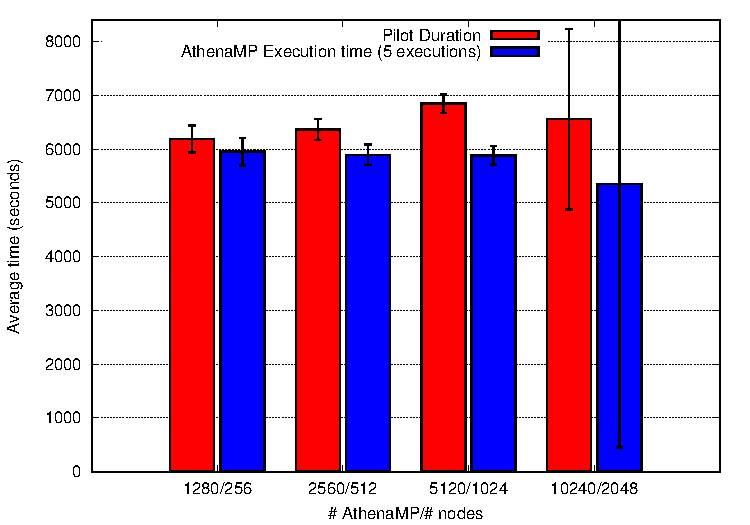
\includegraphics[width=0.5\textwidth]{./figures/NGE/weakET2.pdf}
    \caption{Average pilot execution time against average AthenaMP execution times  for pilot sizes: 256, 512, 1024 and 2048.}
\label{fig:weakScal2a}
\end{figure}
\begin{figure}[!htb]
        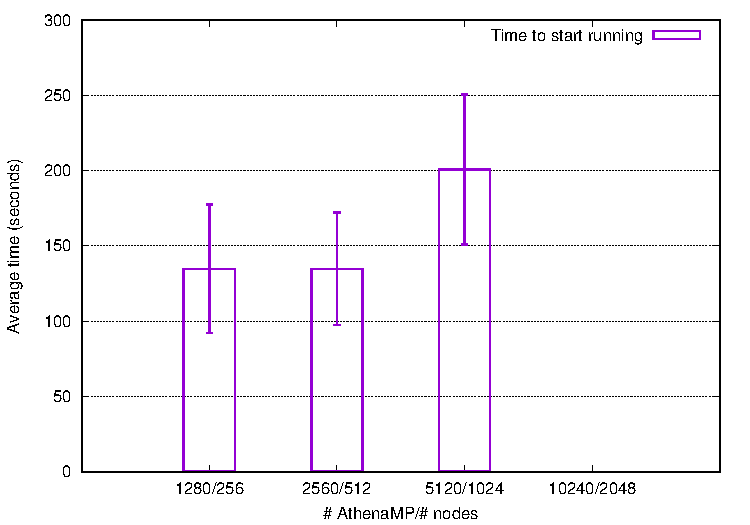
\includegraphics[width=0.5\textwidth]{./figures/NGE/weakStart2.pdf}
    \caption{Average time to start running AthenaMP for pilot sizes: 256, 512, 1024 and 2048.}
\label{fig:weakScal2b}
\end{figure}
\subsubsection{Strong scalability}
This experiments aim to test strong scalability. Therefore, we run the same amount of tasks for different pilot sizes. 
We used a number of AthenaMP instances equal to 2048 and tested pilots with 256, 512, 1024 and 2048 nodes. 
Each AthenaMP instance simulates sixteen events as the previous experiment.

Figure \ref{fig:strongScala} depicts the average pilot duration and  the average execution time of AthenaMP.  

%\begin{figure}[!htb]
%        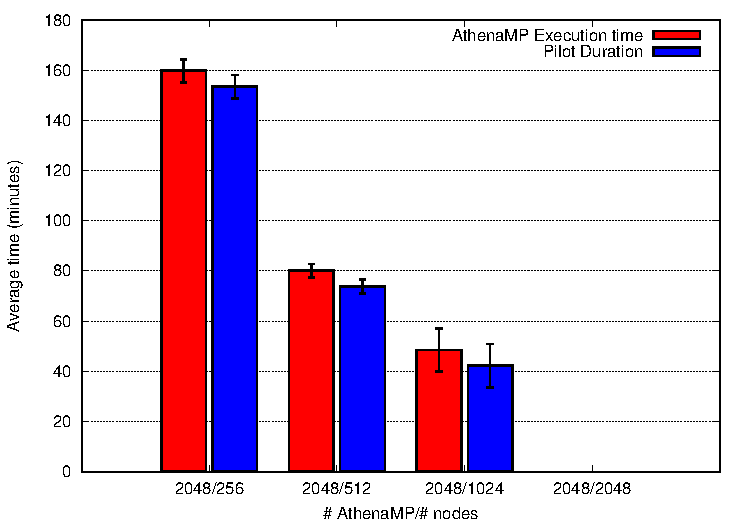
\includegraphics[width=0.5\textwidth]{./figures/NGE/strongET.pdf}
%    \caption{Average pilot execution time against average AthenaMP execution times  for pilot sizes: 256, 512, 1024 and 2048.}
%\label{fig:strongScala}
%\end{figure}
%\begin{figure}[!htb]
%        \includegraphics[width=0.5\textwidth]{./figures/NGE/strongStart.pdf}
%    \caption{Average time to start running AthenaMP for pilot sizes: 256, 512, 1024 and 2048.}
%\label{fig:strongScalb}
%\end{figure}

 
\subsubsection{Heterogeneous execution}

The last experiment provides a proof of concept about the ability of the NGE to execute heterogeneous workload.
In particular, we coupled the execution of AthenaMP with the execution of Gromacs to simulate molecular dynamics. 
We performed the experiment by executing at first one AthenaMP per node and then, submitting a Gromacs simulation per core. Each Gromacs simulation requires ~20 minutes.
We tested the following pilot sizes : 8, 32, 64. 



% For this reason, the second set of the experiments aims to find
%sub-optimal parameters with which we can minimize the trade-off between the size
%of a slot and the time spent in queue waiting for that slot to become available.
%In other words, we aim to minimize the completion time by finding the best
%trade-off between execution time and queue time.
%
%This execution model introduces slot utilization as one of the key factors for
%high-performances. This happens because, in order to minimize the time spent in
%queue, we might asks for slots in advance and, then we could not be able to
%saturate them when they become available. Thus, this strategy requires a new
%functionality that allows the job to receive and execute new events while it is
%already running on the resources. In order to do that we perform the experiments
%by using a new generation executor that implements such functionality.
%
%As last observation, it is important to point out that the percentage of
%utilization of a slot is minor problem with the current implementation because,
%due to the dynamics of the Backfill queue, PanDA has a high probability to
%re-acquire a slot immediately after it has released one\aanote{Are we able to
%quantify this ``immediately''?}.
